\documentclass{article}
\usepackage[utf8]{inputenc}
\setlength{\parindent}{0cm}
\addtolength{\hoffset}{-2cm}
\addtolength{\textwidth}{4cm}
\usepackage[frenchb]{babel}
\usepackage[T1]{fontenc}
\usepackage[hidelinks]{hyperref}
\usepackage{graphicx}
\usepackage{afterpage}
\usepackage{minted}
\usepackage{pdflscape}
\usepackage{pdfpages}

\title{Réseau de Neuroévolution Appliqué au Jeu Vidéo}
\author{Thomas Ibanez}
\makeindex


\begin{document}

\maketitle
\newpage

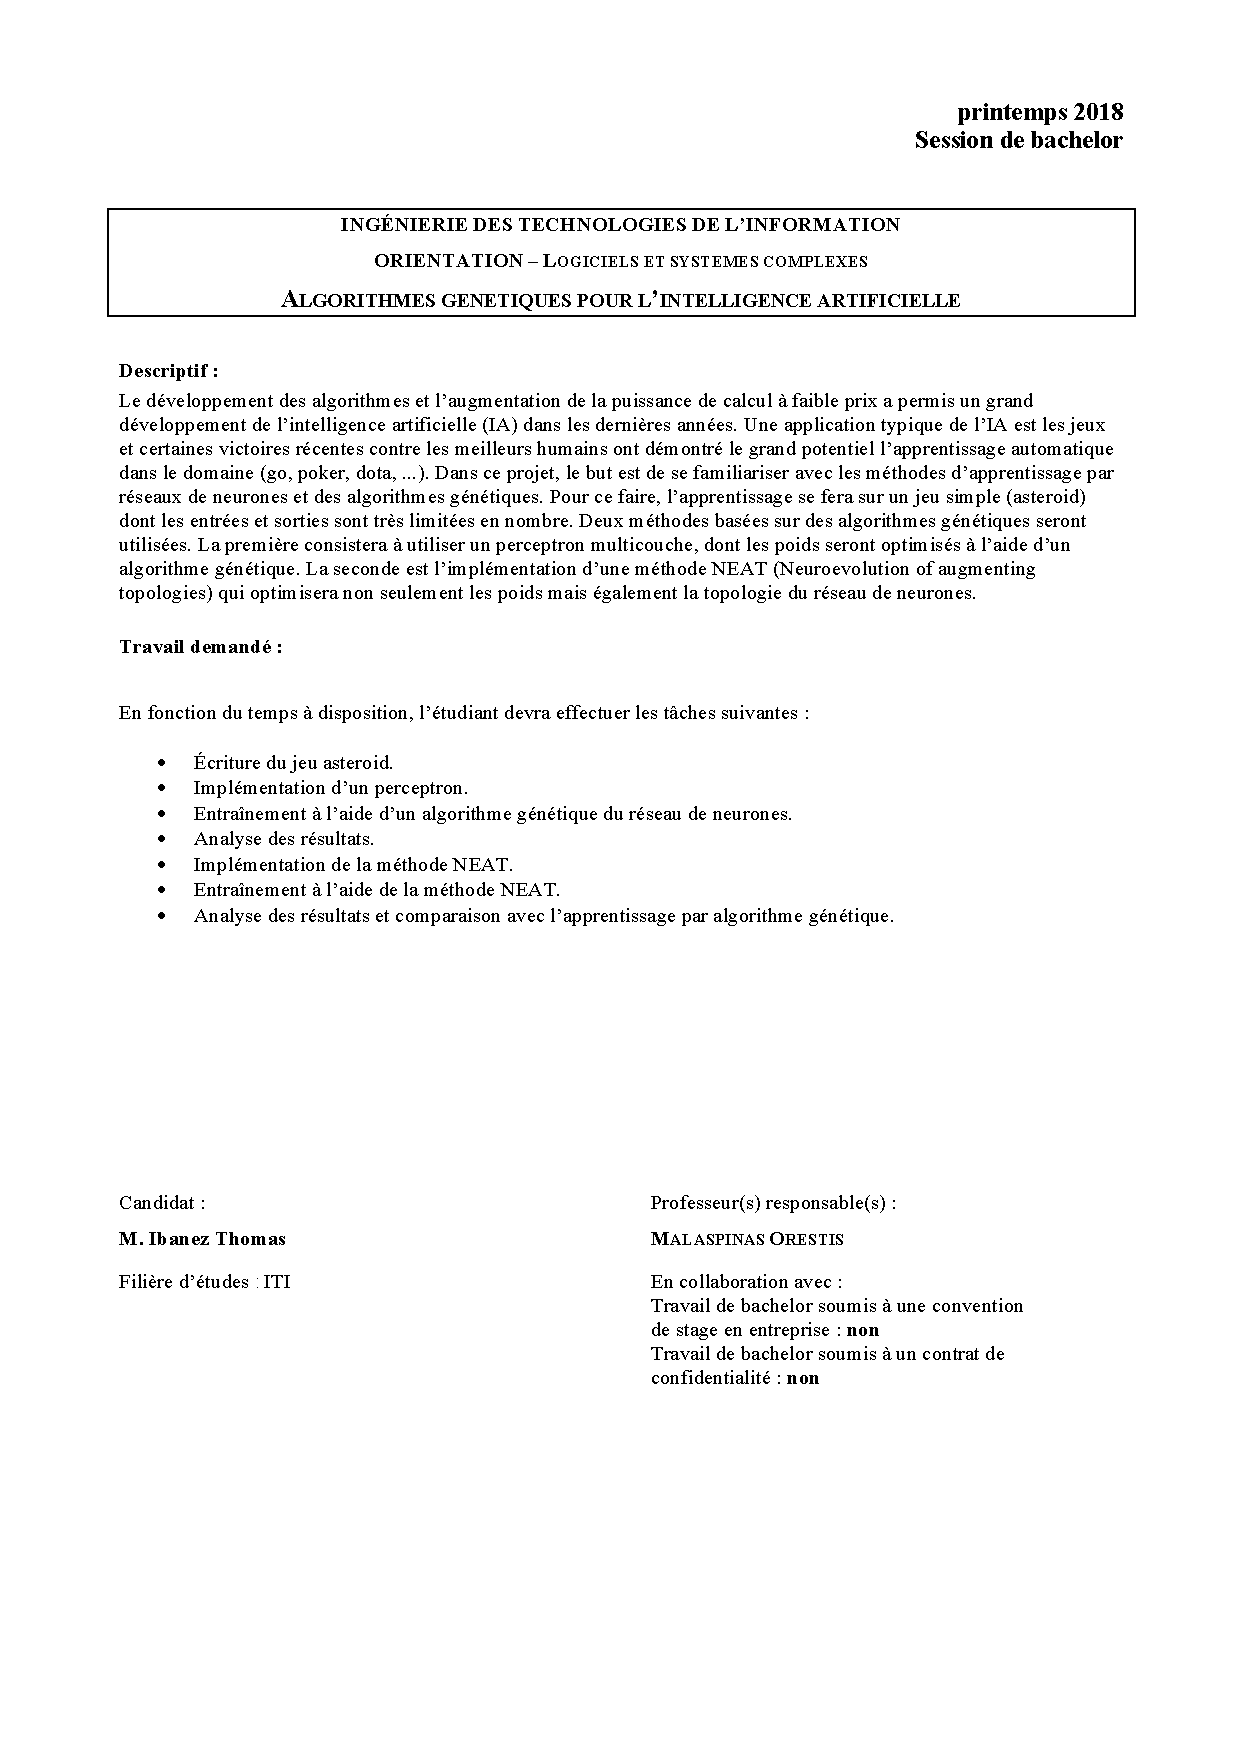
\includepdf[pages=1, offset=2cm 0]{enonce}

\tableofcontents

\newpage

\listoffigures

\newpage

\section*{Remerciements}
\section*{Acronymes}
IA
NEAT


\newpage
\section{Introduction}

Ces dernières années l'apprentissage automatique (Machine Learning) à pris une place très importante dans le monde de l'informatique et nous avons pu assister au prouesses accomplies par des intelligences artificielles tels que la victoire d'AlphaGo face à Lee Sedol au jeu de Go en 2016.\cite{wikialphagolee} Cet événement n'est pas sans rappeler la defaite de Kasparov contre Deep Blue en 1997 qui avait défrayé le chronique.\cite{kasparov}\\
Mais comment en sommes nous arrivés là, et quels sont les techniques qui se cachent derrière ces impressionnant résultats ?\\
Il y a plusieurs manière de faire du machine learning ; une des plus populaire, celle qui est utilisée pour ce travail, est le réseau de neurones artificiels. Cette technologie existe depuis bien longtemps, mais ce sont les récent progrès en terme de puissance de calcul qui ont amorcé sa montée comme technologie phare du domaine.\cite{nnpower}\\

La méthode classique pour entrainer des réseaux de neurones est la rétropropagation du gradient (backpropagation). Cette technique consiste à comparer la sorties du réseau à la sortie attendu pour une entrée donnée afin de corriger les poids du réseau.\cite{backprop} L'avantage de cette technique est qu'elle va converger très rapidement vers le résultat attendu (à condition que les hyperparamètres du réseau soit adaptés au problème). Le désavantage est qu'il faut avoir à sa disposition un grand nombres d'entrées dont on connait la nature afin de pouvoir les comparer aux résultats du réseau. Par exemple il existe une base de données de chiffres écrit à la main avec leur valeur réelle sur \url{http://yann.lecun.com/exdb/mnist/} (70'000 entrées).\\

Cependant générer une telle base de données est un travail énorme, ainsi ces dernières années nous avons assisté à l'émergence de nouvelles technique ne nécessitant pas d'exemples.\\

Une de ces techniques, qui a été utilisée pour l'apprentissage d'AlphaGo\cite{alphago}, est le l'apprentissage par renforcement (Reinforcement learning). Cette méthode consiste à juger les décisions prises par un agent autonome en lui donnant une recompense positive ou négative afin que l'agent, au fur et à mesure des expériences trouve une stratégie optimale.\cite{wikirl} Cette façon de faire peut être comparé au comportement d'un enfant qui apprends à faire du vélo. Quand il tombe il va avoir mal, c'est une récompense négative. Il va donc corriger son comportement de façon à ne plus tomber. A l'inverse, quand il arrive a aller loin il va être fier et donc favoriser ce comportement, c'est une récompense positive.\\

Cependant il existe une méthode encore plus généraliste pour l'apprentissage: La neuroévolution. Cette méthode se base sur les algorithmes évolutionniste dont le fonctionnement est inspiré de la sélection naturelle qui a guidé l'évolution de la vie sur terre. En effet à partir d'un ensemble d'organismes que nous allons évaluer à leur capacité effectuer une tâche donnée, ce que nous appelons le \textit{fitness} de l'organisme. Nous allons sélectionner les meilleurs d'entre eux afin de les faire se "reproduire" pour créer la génération suivante qui sera à son tour évaluée et on recommence ce processus autant de fois que nécessaire.\cite{wikineuroevolution}\\

Le but de ce travail de bachelor est d'étudier et de comparer le comportement deux algorithmes de neuroévolution en analysant la faculté de chacun à apprendre à jouer à des jeux vidéo. Cette technique à été choisie car elle permet un développement plus libre de l'IA en ne jugeant que le résultat et non pas les actions qui y mène.
\newpage
\section{Réseau de Neurones Artificiels}

Un réseau de neurones est un modèle, inspiré du fonctionnement du cerveau humain, qui va consister en un ensemble de neurones artificiels (aussi appelés perceptrons), disposés en couches qui vont communiquer en propageant une information.\cite{wikiann} En effet les neurones de notre cerveau vont collecter les signaux en provenance de leurs dendrites, puis si les signaux sont assez fort envoyer une impulsion le long de leur axone vers les neurones suivant qui vont faire de même. A noter que les connexions entre deux neurones peuvent être plus ou moins fortes (le signal va donc se propager avec une intensité variable).\cite{neuronswork}

\begin{figure}[h]
\begin{center}
	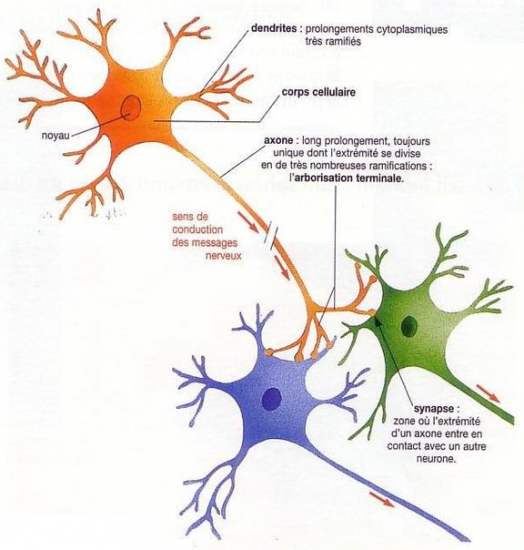
\includegraphics[scale=0.5]{neurones.png}
	\caption{Représentation des neurones dans le cerveau humain \cite{neurons}}
\end{center}
\end{figure}

Les perceptrons quant à eux vont imiter (de manière simplifiée) ce comportement, chaque perceptron va prendre le signal envoyée par chacun de ses voisins de la couche précédente, puis multiplier cette valeur par le poids le connexion et finalement faire le somme de toutes les valeurs pondérées et passer cette somme dans une fonction (dites fonction d'activation) qui va placer cette somme dans un interval (entre 0 et 1 par exemple) et renvoyer le résultat de cette fonction à tous ses voisins de la couche suivante qui vont faire de même.\cite{wikiperceptron}

D'un point de vue mathématique le comportement d'un perceptron peut être écrit comme:
\begin{equation}
o = f(\sum_{i=0}^{n} S_i * W_i)
\end{equation}
Où\\
$o$ est le signal qui va sortir du perceptron\\
$f$ est la fonction d'activation\\
$n$ est le nombre de voisins de la couche précédente\\
$S$ est le vecteur des signaux des voisins la couche précédente\\
$W$ est le vecteur des poids entre le perceptrons et ses voisins de la couche précédente

\begin{figure}[h]
\begin{center}
	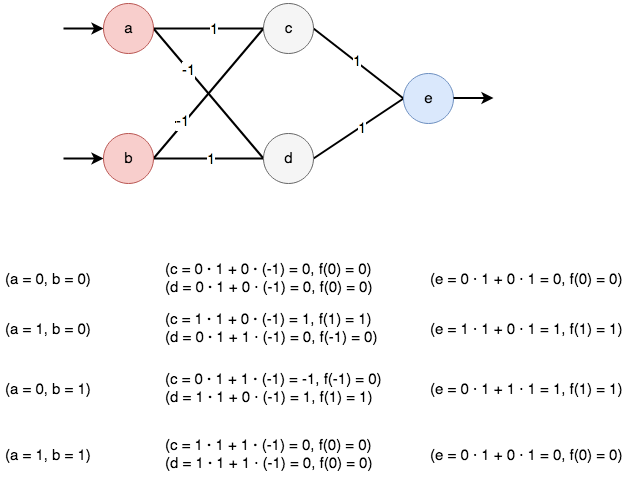
\includegraphics[scale=0.7]{xor.png} 
	\caption{Porte logique "ou exclusif" (XOR) simulée par un réseau de neurones}
\end{center}
\end{figure}

\newpage
\section{Algorithmes évolutionnistes}

Un algorithme évolutionniste est un algorithme d'optimisation métaheuristique qui cherche, par un processus inspiré de la sélection naturelle, une solution optimale à un problème. Ces algorithmes utilisent des iterations stochastiques pour arriver à maximiser une fonction évaluant leurs performances, dite fonction de fitness.\cite{wikiea}\\
Il existe plusieurs sortes d'algorithmes évolutionniste, la neuroévolution en est une et c'est celle-ci qui va nous intéresser. Le but de cette technique est d'utiliser les principes des algorithmes évolutionnistes afin d'optimiser un réseau de neurones pour effectuer la tâche désirée.\\
Les paramètres sur lesquels l'algorithme va intervenir peuvent être les poids des connexions dans le réseau ainsi que la topologie du réseau (nombre de neurones, connexions entre chaque neurones, nombre de couches).

\subsection{Génome \& Phénome}

Le génome est l'ensemble du matériel génétique d'un individu, celui-ci contient toutes les informations nécessaire à la création de l'individu.\cite{wikigenome} Chez les humain le génome est organisé en 23 paires de chromosomes. A partir de ces chromosomes, qui sont uniques à chaque organismes, on peut créer le phénome.\\
Le phénome est l'ensemble de tout les traits observables chez un individu (p.ex La couleur des yeux, de la peau, des cheveux etc...).\cite{wikiphenome}\\

Dans le cadre de la neuroévolution le génome est un encodage permettant la création du phénome qui est le réseau de neurones.

\subsection{Population initiale}

La base d'un algorithme évolutionniste est la population initiale, celle-ci doit être générée aléatoirement afin de représenter un vaste spectre de possibilités. 
Nous ne retrouverons dans cette population aléatoire aucuns individu capable d'accomplir parfaitement la tâche demandée, mais certains aurons des comportements qui les aiderons a d'obtenir un fitness plus élevé que leurs voisins, ceux-ci vont donc passer leurs caractéristiques à la génération suivante.

\subsection{Sélection}

La sélection est un concept essentiel dans l'utilisation d'algorithmes évolutionnistes. L'objectif est de choisir, en prenant en compte le fitness afin que les individus performant soit plus souvent sélectionnés pour être parents. Ainsi, les caractéristiques qui les rendent plus performant seront plus largement passés vers la génération suivante alors que les caractéristiques des individus plus faibles disparaîtront rapidement.\cite{wikifps}

\begin{figure}[h]
\begin{center}
	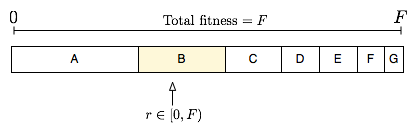
\includegraphics[scale=0.6]{fps.png} 
	\caption{Exemple de sélection proportionnelle au fitness\cite{wikifps}}
\end{center}
\end{figure}
\newpage

\subsection{Crossover}

Un crossover (où enjambement en français) est une opération génétique qui croise les gènes de deux parents afin de créer le gène de l'enfant, ce dernier va donc hériter de certaines caractéristiques de l'un où l'autre parent. Un exemple visible de cette opération chez les humains est que l'on reconnait des traits (couleur de peau, yeux, cheveux) des parents chez les enfants.\cite{wikicrossover}\\

\subsection{Mutation}

Les mutations sont des événements aléatoires qui vont altérer le génome de façon à créer une innovation, qui va par exemple se traduire par un comportement différent du génome. Dans certains cas les mutations seront bénéfiques (p.ex La capacité à respirer hors de l'eau), dans d'autre la mutation causera un comportement désavantageux (p.ex Malformation des membres).\cite{wikimutation}\\

\subsection{Elitisme}

L'Elitisme est un concept qui va permettre la survie des meilleurs individus d'une génération vers la génération suivante sans que leur code génétique soit modifié.\cite{elitism}\\
La raison pour laquelle ce concept est mis en place est que les solutions optimales trouvées ne doivent pas être perdues à cause de mutations désavantageuses.


\newpage
\section{Evolution du perceptron multicouche - Algorithme Naïf}

Cette section détaille le fonctionnement de l'algorithme évolutionniste mis en place pour faire évoluer les perceptrons multicouche à topologie fixe. Celui-ci va donc uniquement faire varier les poids des connexion dans le réseau pour optimiser son comportement. L'algorithme à été créé en s'inspirant des concepts d'algorithmes évolutionnistes décrit précédemment.

\subsection{Génome \& Phénome}

Pour cet algorithme le génome est simplement la liste des poids constituant le réseau de neurones. Ainsi, étant donne que la topologie du réseau est fixe, on peut le reproduire à l'identique en assignant les bons poids.\\

Le phénome dans le cas de cet algorithme sera une réseau de neurones à topologie fixe et entièrement connecté (Chaque neurones d'une couche donnée est connecté a chaque neurones de la couche suivante).

\begin{figure}[h]
\begin{center}
	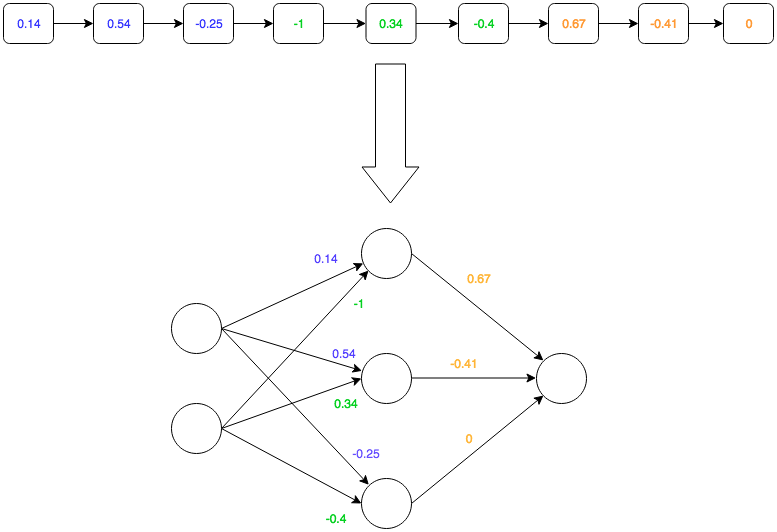
\includegraphics[scale=0.5]{genomephenome.png}
	\caption{Passage du génome au phénome}
\end{center}
\end{figure}

\subsection{Population initiale}

La population initiale est un ensemble de perceptrons multicouche dont la topologie est la même, les poids entre les couches sont assignés aléatoirement à une valeur entre -1 et +1 afin de représenter un spectre de possibilités aussi large que possible.
\begin{figure}[h]
\begin{center}
	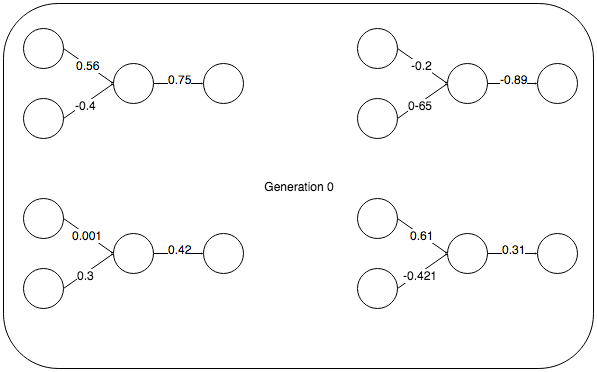
\includegraphics[scale=0.6]{gen0mlp.png} 
	\caption{Exemple de population initiale}
\end{center}
\end{figure}

\subsection{Sélection}

La sélection est utilisée pour choisir un individu de la génération précédente qui va soit passer ses gènes directement (être cloné), soit faire un crossover avec les gènes d'un autre individu lui aussi sélectionné. La probabilité de l'une ou l'autre de ces actions est de 50\%.\\
Le génome résultant de cette sélection subira ensuite une potentielle mutation. Ce processus est répété autant de fois que nécessaire pour créer une nouvelle génération contenant autant d'organismes que la précédente.

\subsection{Crossover}

Le crossover fonctionne d'après un principe très simple:\\
\begin{itemize}
\item Choisir un point de croisement
\item Assigner chez l'enfant tout les gènes qui précèdent ce point depuis le premier parent
\item Assigner chez l'enfant tout les gènes qui suivent ce point depuis le second parent
\end{itemize}

\begin{figure}[h]
\begin{center}
	\includegraphics[scale=0.6]{"crossover.png"} 
	\caption{Fonctionnement d'un crossover}
\end{center}
\end{figure}
\newpage

Ainsi, les traits permettant une meilleure survie vont rapidement se répandre dans la population car les individus ayant obtenu un meilleur fitness serons plus souvent sélectionnés pour faire une crossover avec un autre individu.

\subsection{Mutation}

Dans le cas de cet algorithme, étant donné que la topologie est fixe, la mutation sera simplement une variation aléatoire d'un poids dans le réseau de neurones. Ainsi chaque enfant de chaque génération aura 10\% de chance que l'un de ses gènes subisse une mutation.\\
Le poids subira donc une variation d'une valeur aléatoire choisie entre +0.5 et -0.5 cependant le poids sera ensuite fixée dans l'interval $[-1, 1]$.

\begin{figure}[h]
\begin{center}
	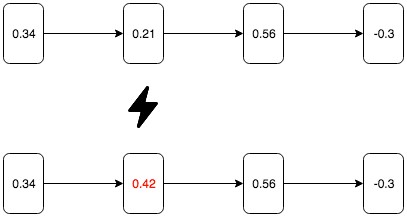
\includegraphics[scale=0.6]{mutation.png}
	\caption{Exemple de mutation dans un génome}
\end{center}
\end{figure}
\newpage

\subsection{Elitisme}

Pour cet algorithme, seul le champion de la génération (organisme ayant obtenu le meilleur fitness) est préservé sans altération de son code génétique pour la génération suivante.

\begin{figure}[h]
\begin{center}
	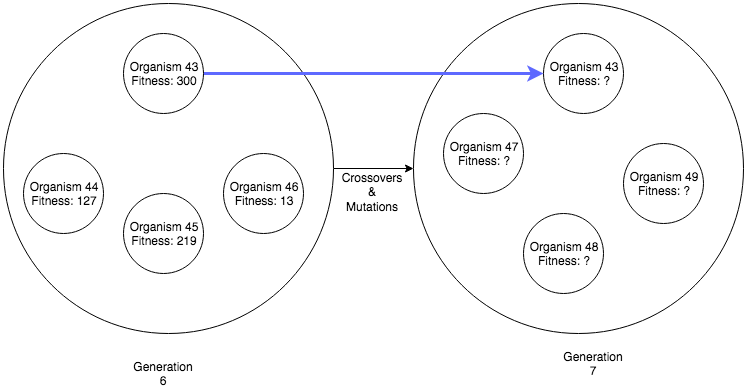
\includegraphics[scale=0.5]{elitism.png}
	\caption{Elitisme d'une génération vers la suivante}
\end{center}
\end{figure}

\subsection{Déroulement de l'algorithme}

L'organigramme ci-dessous décrit le comportement global de l'algorithme. La fonction random(0, 1) va tirer un nombre aléatoire entre compris dans l'interval $[0, 1[$.
\afterpage{%
\begin{figure}[!htbp]
\centering
\vspace*{-3cm}
\thispagestyle{empty}
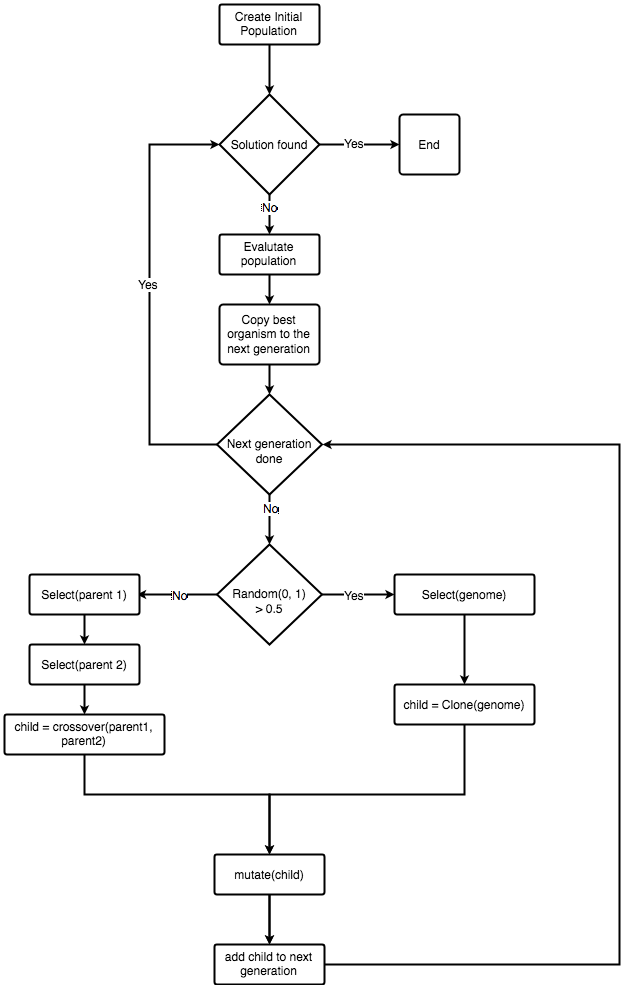
\includegraphics[scale=0.6]{mlporga.png}
\caption{Organigramme de l'algorithme naïf}
\end{figure}
\clearpage
}
\newpage

\section{NEAT}

L'autre algorithme de neuroévolution mis en place est le NEAT, créé par Ken Stanley à Université du Texas à Austin. Cet algorithme détaille comment obtenir des réseaux de neurones dont la topologie change au fil des évolutions.\\
Il apporte trois techniques essentielles à son fonctionnement: suivre l'évolution des gènes avec un historique pour permettre les crossover parmi les différentes topologies, séparer les organismes en espèces afin de préserver l'innovation et faire évoluer les topologies de manière incrémentale en partant de structures simples afin d'obtenir des résultats minimaux.\cite{wikineat}

\subsection{Génome \& Phénome}

Dans le cas de NEAT, le génome est plus complexe, en effet il doit représenter tout les neurones et toutes les connexions. 

\subsection{Population initiale}

La population initiale doit être aussi simple que possible, cependant il n'y a pas de règles dictant la manière dont elle doit être faite. Pour cet algorithme, la population initiale est donc un ensemble de perceptron multicouche avec seulement une couche d'entrée et une couche de sortie dans lequel chaque entrée est reliée à chaque sorties.

\begin{figure}[h]
\begin{center}
	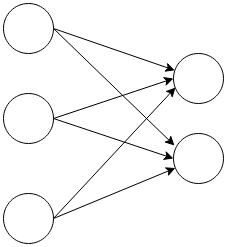
\includegraphics[scale=0.6]{initneat.png}
	\caption{Exemple de population initiale dans NEAT}
\end{center}
\end{figure}

Ce choix à été fait pour conserver un équilibre entre une population simple (pas de couche intermédiaire) mais qui soit rapidement capable de s'ajuster car les connexions sont déjà disponibles, on ne pert donc pas de générations uniquement pour créer les connexions.

\subsection{Spéciation}

\subsection{Sélection}


\subsection{Crossover}

Le crossover dans le cadre du NEAT pose le problème des conventions concurrentes (competing conventions). En effet il possible que deux réseaux produisent le même résultat mais de manière différente, le risque est que lorsque nous croisons les deux réseau nous perdions une partie de l'information qui les rends efficace.

\begin{figure}[h]
\begin{center}
	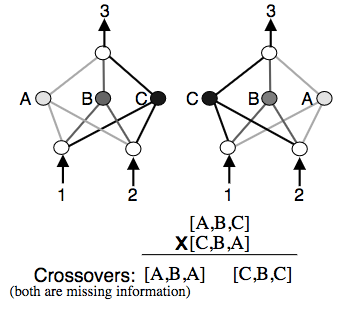
\includegraphics[scale=0.5]{competingconventions.png}
	\caption{Problème des conventions concurrentes, les deux réseaux atteignent le même résultat mais leurs possibles enfants en n'aurons que 2/3 de l'information \cite{neatpaper}}
\end{center}
\end{figure}
\newpage

Afin de pallier à ce problème, nous suivons l'apparitions d'innovations, 

\subsection{Mutation}
\subsection{Elitisme}

\newpage
\section{Architecture Réseau}

Afin d'optimiser la vitesse de calcul, un système distribué à été mis en place. Celui-ci repose sur une architecture client-serveur classique où le client effectue les simulations et le serveur gère les génomes et s'occupe de distribuer de manière équitable le travail entre tous les clients.\\

\subsection{Protcole}

Le protocole à été établi à l'aide du langage protobuf qui permet d'avoir une définition claire ne dépendant pas des langages dans lesquels le protcole est ensuite implémenté.

Voici le fichier qui défini le protocole:
\inputminted[breaklines,breaksymbol=, frame=single,label=Protocole, stepnumber=1,tabsize=2]{protobuf}{mg.proto}

Le protocole définit donc 6 types de messages:
\begin{itemize}
\item MG\_JOIN, Envoyé par le client, c'est une demande à rejoindre le groupe de calcul. En paramètres sont donnés le nom du client et si il veut rejoindre en tant que specateur ou non (fonctionnalité expliquée dans la partie client).

\item MG\_JOIN\_RESPONSE, Envoyé par le serveur, confirme ou infirme l'ajout au groupe du client. Il n'existe pour l'instant aucune raison pour le rejet d'un client.

\item MG\_COMPUTE\_REQUEST, Envoyé par le serveur, demande au client de calculer le fitness d'un génome donné sur un jeu donné.

\item MG\_COMPUTE\_RESPONSE, Envoyé par le client, indique au serveur si oui ou non le client est en mesure d'effectuer la simulation.

\item MG\_COMPUTE\_RESULT, Envoyé par le client, donne le fitness obtenu par le génome donné dans le message MG\_COMPUTE\_REQUEST sur le jeu donné dans ce même message et le temps (ms) pris par le client pour effectuer la simulation.

\item MG\_END, Envoyé par n'importe quel entité, indique un désir de terminer la connexion.

\end{itemize}

\subsection{Serveur}

Comme écrit ci-dessus, le serveur à la lourde tâche de gérer tous les génomes et leurs fitness afin de mettre en oeuvre les algorithmes évolutionniste qui vont permettre l'évolution. En plus de cela il va également devoir servir les pages web servant à la gestion et à la surveillance du processus évolutif.\\
Afin de pouvoir effectuer toutes ces tâches, le serveur est constitué de modules node.js qui vont chacun gérer une partie de ce qui est lui est demandé.\\
L'architecture se présente ainsi:
\begin{figure}[h]
\begin{center}
	\includegraphics[scale=0.5]{"server.png"} 
	\caption{Architecture des modules du serveur}
\end{center}
\end{figure}
\newpage

\subsection{Client}

Le client va devoir effectuer la simulation demandée par le serveur, avec le bon réseau de neurones

\subsubsection{Réseaux de neurones}
\subsubsection{Simulateur}
\subsubsection{Tests}

\newpage
\section{Interface de Controle}
\subsection{Mode}
\subsection{Tâche}
\subsection{Ouvriers}
\subsection{Graphs}

\newpage
\section{Base de donnés}

\newpage
\section{API}

\newpage
\section{Jeux}
\subsection{Asteroid}
\subsubsection{Principe}
\subsubsection{Entrées}
\subsubsection{Sorties}
\subsubsection{Résultats}

\newpage
\section{Conclusion}

\newpage
\bibliographystyle{unsrt}
\bibliography{mg}
\end{document}
